 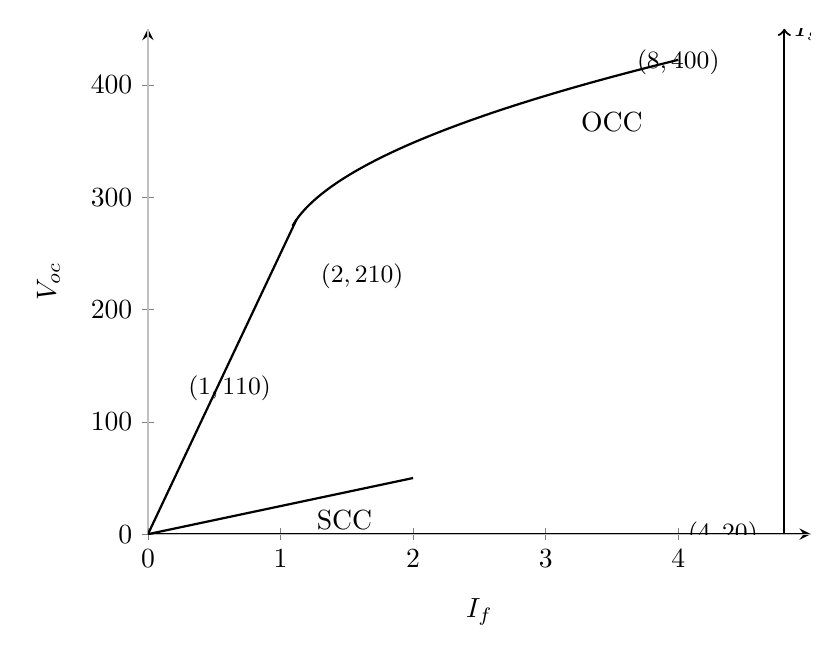
\begin{tikzpicture}
        \begin{axis}[
            axis lines = middle,
            xlabel = $I_f$,
            ylabel = $V_{oc}$,
            xmin = 0, xmax = 5,
            ymin = 0, ymax = 450,
            xtick = {0,1,2,3,4},
            ytick = {0,100,200,300,400},
            x label style={at={(axis description cs:1,0)},anchor=west},
            y label style={at={(axis description cs:0,1)},anchor=south},
            extra x ticks={0},
            extra y ticks={0},
            extra tick style={grid=major},
            axis line style=thick,
            xlabel near ticks,
            ylabel near ticks,
            every axis plot/.append style={thick},
            legend pos = north west,
            width=10cm, height=8cm,
        ]
        \addplot[domain=1.09:4, samples=100, smooth] {100*(x-1.03)^(0.5)+250};
        \addplot[domain=0:2, samples=2] {25*x};
        \addplot[domain=0:1.12, samples=2] {250*x};
        \node at (axis cs:0,0) [below left] {\small $(0,0)$};
        \node at (axis cs:0,10) [left] {\small $(0,10)$};
        \node at (axis cs:1,110) [above left] {\small $(1,110)$};
        \node at (axis cs:2,210) [above left] {\small $(2,210)$};
        \node at (axis cs:4,20) [below right] {\small $(4,20)$};
        \node at (axis cs:4,400) [above] {\small $(8,400)$};
        \node at (axis cs:3.5,350) [above] {OCC};
        \node at (axis cs:1.2,30) [below right] {SCC};
        \draw[->, thick] (axis cs:4.8,0) -- (axis cs:4.8,450) node [right] {$I_{sc}$};
        \node[above] at (axis cs:0,450) {$V_{oc}$};
        \end{axis}
    \end{tikzpicture}
   
